\documentclass[11pt,oneside]{article}

\usepackage[a4paper,margin=26mm,headheight=15pt]{geometry}
\usepackage[T1]{fontenc}
\usepackage[utf8]{inputenc}
\IfFileExists{libertinus.sty}{\usepackage{libertinus}}{\usepackage{lmodern}}
\usepackage{microtype}
\usepackage{amsmath,amssymb,amsthm,mathtools,mathrsfs,bm}
\usepackage{booktabs,longtable,array,tabularx,multirow}
\usepackage{graphicx}
\usepackage{xcolor}
\usepackage{enumitem}
\usepackage{fancyhdr}
\usepackage{titlesec}
\usepackage{listings}
\usepackage{xurl}
\usepackage{hyperref}
\usepackage[nameinlink,noabbrev]{cleveref}

\definecolor{linkblue}{RGB}{25,75,135}
\definecolor{shadegray}{RGB}{246,247,249}
\definecolor{rulegray}{RGB}{195,201,208}
\hypersetup{
  colorlinks=true,
  linkcolor=linkblue,
  citecolor=linkblue,
  urlcolor=linkblue,
  pdftitle={Exact Polynomial Plateaux from Rvachev's Up-Function},
  pdfauthor={Research report prepared for Vladimir Reshetnikov},
  pdfsubject={Exact finite representations of polynomials by shifted and scaled Rvachev up-functions},
  pdfkeywords={Rvachev up-function, Fabius function, polynomial reproduction, Strang-Fix, Appell polynomials, Bell polynomials, Bernoulli numbers, Thue-Morse sequence, sinc product}
}

\pagestyle{fancy}
\fancyhf{}
\fancyhead[L]{\small Exact up-polynomial plateaux}
\fancyhead[R]{\small\nouppercase{\leftmark}}
\fancyfoot[C]{\thepage}
\renewcommand{\headrulewidth}{0.4pt}
\titleformat{\section}{\Large\bfseries}{\thesection}{0.7em}{}
\titleformat{\subsection}{\large\bfseries}{\thesubsection}{0.7em}{}
\titleformat{\subsubsection}{\normalsize\bfseries}{\thesubsubsection}{0.7em}{}
\setcounter{secnumdepth}{3}
\setcounter{tocdepth}{2}
\setlist[itemize]{leftmargin=2em,itemsep=0.28em,topsep=0.45em}
\setlist[enumerate]{leftmargin=2.4em,itemsep=0.28em,topsep=0.45em}
\setlength{\emergencystretch}{3em}

\newtheorem{theorem}{Theorem}[section]
\newtheorem{proposition}[theorem]{Proposition}
\newtheorem{lemma}[theorem]{Lemma}
\newtheorem{corollary}[theorem]{Corollary}
\newtheorem{conjecture}[theorem]{Conjecture}
\theoremstyle{definition}
\newtheorem{definition}[theorem]{Definition}
\newtheorem{algorithm}[theorem]{Algorithm}
\newtheorem{example}[theorem]{Example}
\theoremstyle{remark}
\newtheorem{remark}[theorem]{Remark}
\newtheorem{warning}[theorem]{Warning}

\newcommand{\R}{\mathbb R}
\newcommand{\C}{\mathbb C}
\newcommand{\Q}{\mathbb Q}
\newcommand{\N}{\mathbb N}
\newcommand{\Z}{\mathbb Z}
\newcommand{\Up}{\operatorname{up}}
\newcommand{\sinc}{\operatorname{sinc}}
\newcommand{\supp}{\operatorname{supp}}
\newcommand{\E}{\mathbb E}
\newcommand{\Var}{\operatorname{Var}}
\newcommand{\wt}{\operatorname{wt}_2}
\newcommand{\vtwo}{\nu_2}
\newcommand{\dd}{\,\mathrm d}
\newcommand{\e}{\mathrm e}
\newcommand{\ii}{\mathrm i}
\newcommand{\D}{\mathrm D}
\newcommand{\Id}{\operatorname{Id}}
\newcommand{\Span}{\operatorname{span}}
\newcommand{\bigO}{\mathcal O}
\newcommand{\smallo}{o}
\newcommand{\floor}[1]{\left\lfloor #1\right\rfloor}
\newcommand{\ceil}[1]{\left\lceil #1\right\rceil}
\newcommand{\abs}[1]{\left|#1\right|}
\newcommand{\norm}[1]{\left\lVert#1\right\rVert}
\newcommand{\set}[1]{\left\{#1\right\}}
\newcommand{\coeff}[2]{\left[#1^{#2}\right]}
\newcommand{\repo}{\nolinkurl{Analysis/FabiusFunction/docs}}
\newcommand{\qbinom}[3]{\genfrac{[}{]}{0pt}{}{#1}{#2}_{#3}}

\newenvironment{resultbox}{%
  \par\smallskip\noindent\begin{center}\begin{minipage}{0.94\textwidth}%
  \hrule\vspace{0.6em}\small
}{%
  \vspace{0.6em}\hrule\end{minipage}\end{center}\smallskip
}
\newenvironment{conjecturebox}{%
  \par\smallskip\noindent\begin{center}\begin{minipage}{0.94\textwidth}%
  \hrule\vspace{0.6em}\small
}{%
  \vspace{0.6em}\hrule\end{minipage}\end{center}\smallskip
}

\lstdefinestyle{pseudo}{
  basicstyle=\ttfamily\small,
  backgroundcolor=\color{shadegray},
  frame=single,
  rulecolor=\color{rulegray},
  columns=fullflexible,
  keepspaces=true,
  showstringspaces=false,
  xleftmargin=0.7em,
  xrightmargin=0.7em,
  aboveskip=0.8em,
  belowskip=0.8em
}

\title{\bfseries Exact Polynomial Plateaux from Rvachev's Up-Function\\[0.35em]
\large Dyadic oversampling, Appell deconvolution, finite interval algorithms,\\
Thue--Morse antiderivatives, and sharp reproduction order}
\author{Research report prepared for Vladimir Reshetnikov}
\date{Repository snapshot: commit \texttt{5915d9a723c9ae01a2cc4be8a251bdcb11d9e406}\\28 August 2026}

\begin{document}
\maketitle

\begin{abstract}
Let \(\Up\) denote Rvachev's even \(C^\infty\) compactly supported function on
\([-1,1]\), normalized by \(\int\Up=1\).  This report gives an explicit exact
solution of the following problem: for an arbitrary polynomial \(p\) and a
prescribed compact interval \(I=[A,B]\), construct a finite sum of shifted and
scaled copies of \(\Up\) agreeing with \(p\) at every point of \(I\).

The construction is stronger than existence.  All atoms may have one common
horizontal scale.  Choose an integer oversampling ratio \(m\) with
\(\vtwo(m)\ge\deg p\), a lattice step \(h>0\), and centers
\(x_k=x_0+kh\).  Put \(\rho=mh\), let
\[
 M(z)=\int_\R \e^{zx}\Up(x)\,\dd x
     =\prod_{j=1}^{\infty}\frac{\sinh(z/2^j)}{z/2^j},
\]
and define the polynomial deconvolution
\[
 p_\rho^\sharp=M(\rho\D)^{-1}p.
\]
Then the locally finite identity
\[
 p(x)=\frac1m\sum_{k\in\Z}p_\rho^\sharp(x_0+kh)
       \Up\!\left(\frac{x-x_0-kh}{\rho}\right)
\]
holds on all of \(\R\).  Keeping only atoms whose supports meet \(I\) gives
the requested finite formula.  The inverse operator terminates on polynomials
and has rational coefficients expressible through Bernoulli cumulants and
complete Bell polynomials; no collocation system or numerical inversion is
needed.

A twisted Poisson argument proves that the exact stationary reproduction degree
is precisely \(\vtwo(m)\).  Hence the smallest integer ratio in this
common-scale lattice scheme is \(m=2^{\deg p}\).  The first failed degree has
an explicit nonzero Fourier-series defect.  A complementary real-space
construction repeatedly integrates finite \(\Up\)-sums through the
scale-difference identity for \(\Up'\); invisible ``ghost'' atoms repair the
finite zero-sum compatibility conditions and control constants of integration.
Iteration yields an exact Thue--Morse derivative stencil.  The report also
treats finite sinc products, arithmetic, support, conditioning, multivariate
tensor products, conjectures, and future directions.  The accompanying Python
program uses exact rational arithmetic: its 49-atom degree-four example has
residual exactly zero at 129 dyadic points, and seven additional degree tests
from zero through six also return exact zero.
\end{abstract}

\tableofcontents
\newpage

\section{Scope, corpus audit, and status of the results}

\subsection{Repository corpus examined}

The final pinned repository snapshot contains 97 LaTeX sources under \repo,
at commit
\[
 \texttt{5915d9a723c9ae01a2cc4be8a251bdcb11d9e406}.
\]
The tree advanced during preparation, so the audit was refreshed from the
earlier 85-source checkpoint.  The twelve added sources comprise three
independent dyadic-comb reports, two global-interpolation reports, and small
generated or reconstructed TeX fragments.  The inventory otherwise includes
polished syntheses, archived versions, source-paper transcriptions, a
mathematical glossary, Lean walkthroughs, and the large non-formalized frontier
compilation.  Corpus-wide searches and close reading covered:
\begin{itemize}
  \item the normalizations of the bounded Fabius function, its signed global
        extension, and Rvachev's \(\Up\);
  \item support, positivity, endpoint flatness, and the functional-differential
        equation for \(\Up\);
  \item the infinite sinc product for \(\widehat\Up\), its integer zeros, and
        their exact dyadic multiplicities;
  \item Poisson summation, partition-of-unity identities, oversampled
        translate sums, shifted dyadic-comb quadrature, and alias defects;
  \item Kabaya--Iri and centered Rvachev--Appell polynomials, inverse moment
        operators, Bell--Bernoulli formulae, and self-sampling identities;
  \item exact dyadic values, Thue--Morse cancellation, finite convolution
        splines, interpolation, approximation, and frontier proposals.
\end{itemize}

The refreshed nonduplication boundary is important.  The consolidated
\emph{Inverse and Sampling Frontiers} volume already develops the centered
Rvachev--Appell inverse, links it to dyadic self-sampling, proves a shifted
Strang--Fix exactness theorem, and analyzes the first alias obstruction
\cite{repo-sampling}.  Those results, together with the Fourier zero
multiplicities, are treated here as corpus inputs rather than rediscoveries.
The newly added comb papers concern quadrature of polynomials against
\(\Up\) or Fabius weights, while the two interpolation papers concern global
equispaced polynomial interpolants; neither constructs a finite sum of
\(\Up\)-atoms that equals a prescribed arbitrary polynomial throughout a
chosen interval.

Relative to that stronger prior-art boundary, the additions developed here
are the interval-synthesis layer: the physical-scale formula for arbitrary
\(p\), explicit finite truncation indices, support and atom-count bounds,
compressed coefficient generation, the sharp common-scale feasibility and
complexity statements, the real-space ghost-antiderivative algorithm, its
Thue--Morse derivative stencil, the finite-sinc-prefix transfer theorem, and
tensor-product extension.  The stationary Appell and alias formulae are
re-derived in the report because they make the construction self-contained,
but are labeled conceptually as prerequisites rather than corpus-relative
novelty.

\subsection{Priority and proof labels}

Polynomial reproduction by integer translates is classical.  The zero
conditions used below belong to the Strang--Fix tradition
\cite{strangfix,dahmenmicchelli,zakharov,deboorron}.  Novelty claims are
therefore deliberately local: ``not found in the inspected ProveIt corpus,''
with emphasis on specialization to the unusual dyadic zero multiplicities of
\(\widehat\Up\), the exact coefficient formulas, and the interval algorithm.
No exhaustive claim over the world literature is made.

Every numbered theorem, proposition, lemma, and corollary below has a proof or
an explicit reduction to a standard cited theorem.  Statements labeled
\emph{Conjecture} are unproved.  Numerical computations only check identities
already derived symbolically.

\section{Normalization and repository inputs}
\label{sec:inputs}

Throughout,
\[
 \widehat f(\xi)=\int_\R f(x)\e^{-2\pi\ii x\xi}\,\dd x,
 \qquad
 \sinc z=\begin{cases}\sin z/z,&z\ne0,\\1,&z=0.\end{cases}
\]
We write \(\phi=\Up\) when emphasizing its role as a generator.

\begin{proposition}[Basic data for \(\Up\)]
\label{prop:basic-data}
The repository normalization satisfies
\begin{align}
 &\phi\in C^\infty(\R),\quad \supp\phi=[-1,1],\quad
   \phi(-x)=\phi(x),\quad \int_\R\phi(x)\,\dd x=1,\label{eq:basic}\\
 &\phi'(x)=2\bigl(\phi(2x+1)-\phi(2x-1)\bigr),\label{eq:up-derivative}\\
 &\widehat\phi(\xi)=\prod_{n=0}^{\infty}
       \sinc\!\left(\frac{\pi\xi}{2^n}\right),\label{eq:fourier-product}\\
 &\sum_{k\in\Z}\phi(t+k)=1.\label{eq:partition}
\end{align}
All derivatives vanish at \(\pm1\), and \(\phi>0\) on \((-1,1)\).
\end{proposition}

These facts are developed in the repository synthesis and by Arias de Reyna
\cite{arias}.  Every translate sum in this report is locally finite because of
compact support.

\begin{proposition}[Integer zero multiplicities]
\label{prop:zeros}
For every nonzero integer \(q\), \(\widehat\phi\) has a zero of exact order
\[
 1+\vtwo(q)
\]
at \(q\).
\end{proposition}

\begin{proof}
The factor indexed by \(n\) in \eqref{eq:fourier-product} vanishes at \(q\)
exactly when \(2^n\mid q\).  Thus the vanishing factors are
\(n=0,1,\ldots,\vtwo(q)\); each zero is simple and all remaining factors are
nonzero.
\end{proof}

\begin{corollary}[Oversampled partition]
\label{cor:oversampled-partition}
For every positive integer \(m\),
\[
 \sum_{k\in\Z}\phi\!\left(\frac{t-k}{m}\right)=m.
\]
\end{corollary}

\begin{proof}
Poisson summation gives Fourier modes
\(m\widehat\phi(mn)\e^{-2\pi\ii nt}\).  The zero mode is \(m\), and all
nonzero modes vanish by \Cref{prop:zeros}.
\end{proof}

\section{The exact interval problem}

\subsection{What is and is not possible}

Given \(p\in\R[x]\) and \(I=[A,B]\), seek constants \(c_j\), centers \(b_j\),
and scales \(a_j>0\) such that
\begin{equation}
 p(x)=\sum_{j=1}^{N}c_j\phi\!\left(\frac{x-b_j}{a_j}\right)
 \qquad(x\in I).
 \label{eq:problem}
\end{equation}
Equality means functional equality at every point, not interpolation at a
finite set of nodes.

\begin{proposition}[Global finite-support obstruction]
\label{prop:global-obstruction}
A finite sum of shifted and scaled copies of \(\phi\) cannot equal a nonzero
polynomial on all of \(\R\).
\end{proposition}

\begin{proof}
A finite sum of compactly supported functions is compactly supported, whereas a
nonzero polynomial is not.
\end{proof}

The interval is therefore essential.  The correct global object is an infinite
but locally finite lattice sum; compact support makes it finite after
restriction to a compact interval.

\subsection{A stronger target}

All scales will be equal, all centers will lie on one arithmetic lattice, and
all coefficients will be samples of one explicitly computable polynomial.  Put
\[
 x_k=x_0+kh,\qquad \rho=mh,
\]
where \(h>0\) is the center spacing and \(m\in\N_{>0}\) is the integer ratio of
atom radius to spacing.  The atoms are
\[
 \phi_{\rho,k}(x)=\phi\!\left(\frac{x-x_k}{\rho}\right).
\]
At any fixed \(x\), at most \(2m+1\) atoms are nonzero.

\section{Moment-generating product and Bernoulli cumulants}
\label{sec:mgf}

Define
\begin{equation}
 M(z)=\int_\R\e^{zx}\phi(x)\,\dd x.
 \label{eq:M-def}
\end{equation}
Substitution \(\xi=\ii z/(2\pi)\) into \eqref{eq:fourier-product} gives
\begin{equation}
 M(z)=\prod_{j=1}^{\infty}\frac{\sinh(z/2^j)}{z/2^j}.
 \label{eq:M-product}
\end{equation}
The function is even, entire, and satisfies \(M(0)=1\).

\begin{proposition}[Cumulants]
\label{prop:cumulants}
If
\[
 \log M(z)=\sum_{r=1}^{\infty}\kappa_{2r}\frac{z^{2r}}{(2r)!},
\]
then
\begin{equation}
 \boxed{\displaystyle
 \kappa_{2r}=\frac{2^{2r-1}B_{2r}}{r(2^{2r}-1)}}
 \qquad(r\ge1).
 \label{eq:kappa}
\end{equation}
In particular,
\[
 \kappa_2=\frac19,\qquad
 \kappa_4=-\frac{2}{225},\qquad
 \kappa_6=\frac{16}{3969},\qquad
 \kappa_8=-\frac{16}{3825}.
\]
\end{proposition}

\begin{proof}
Use
\[
 \log\frac{\sinh w}{w}
 =\sum_{r\ge1}\frac{2^{2r-1}B_{2r}}{r(2r)!}w^{2r},
\]
insert \(w=z/2^j\), and sum
\(\sum_{j\ge1}2^{-2rj}=1/(2^{2r}-1)\).
\end{proof}

\begin{remark}[Odd denominators]
\label{rem:odd-denominators}
After reduction, every \(\kappa_{2r}\) has odd denominator.  The reduced
denominator of \(B_{2r}\) contains exactly one factor of two, and
\(2^{2r-1}/r\) cancels it.  This yields a clean \(2\)-adic bound for the
reproduction coefficients.
\end{remark}

Let \(\mu_j=\int x^j\phi(x)\,\dd x\).  Moments follow from cumulants by
\begin{equation}
 \mu_0=1,\qquad
 \mu_n=\sum_{j=1}^{n}\binom{n-1}{j-1}\kappa_j\mu_{n-j},
 \label{eq:moment-cumulant}
\end{equation}
with odd \(\kappa_j\) and \(\mu_j\) zero.  The first values are
\[
 \mu_2=\frac19,\quad
 \mu_4=\frac{19}{675},\quad
 \mu_6=\frac{583}{59535},\quad
 \mu_8=\frac{132809}{32531625}.
\]

\section{Twisted Poisson summation}
\label{sec:twisted-poisson}

\begin{lemma}[Twisted Poisson identity]
\label{lem:twisted-poisson}
For \(m\in\N_{>0}\), \(t\in\R\), and \(z\in\C\),
\begin{equation}
 \sum_{k\in\Z}\e^{kz}\phi\!\left(\frac{t-k}{m}\right)
 =m\sum_{n\in\Z}\e^{(z-2\pi\ii n)t}
     M(-mz+2\pi\ii mn).
 \label{eq:twisted-poisson}
\end{equation}
Both sides are entire functions of \(z\).
\end{lemma}

\begin{proof}
For fixed \(t\), the left side is finite.  Set
\(f(x)=\e^{zx}\phi((t-x)/m)\).  At integer frequency \(n\),
\begin{align*}
 \widehat f(n)
 &=\int_\R \e^{zx}\phi\!\left(\frac{t-x}{m}\right)
                 \e^{-2\pi\ii nx}\,\dd x\\
 &=m\e^{(z-2\pi\ii n)t}
   \int_\R\phi(u)\e^{(-mz+2\pi\ii mn)u}\,\dd u\\
 &=m\e^{(z-2\pi\ii n)t}M(-mz+2\pi\ii mn).
\end{align*}
Poisson summation applies because \(f\) is smooth and compactly supported; the
rapid Fourier decay is locally uniform in \(z\), giving an entire right side.
\end{proof}

Let \(\nu=\vtwo(m)\).  At every nonzero frequency \(n\),
\(M(2\pi\ii mn)\) has zero order
\[
 1+\vtwo(mn)\ge\nu+1.
\]
Consequently all nonzero aliases in \eqref{eq:twisted-poisson} have zero Taylor
jets through order \(\nu\) at \(z=0\).  This observation drives all exact
polynomial identities below.

\section{The up-Appell polynomials}
\label{sec:appell}

The centered Appell inverse and its mean-value interpretation belong to the
current repository corpus \cite{repo-sampling}; this section fixes the precise
normalization needed for the interval synthesis and derives the coefficient
forms used by the algorithm.

\begin{definition}[Up-Appell sequence]
\label{def:appell}
For a positive integer \(m\), define \(A_r^{(m)}(u)\) by the germ at \(z=0\)
\begin{equation}
 \boxed{\displaystyle
 \sum_{r=0}^{\infty}A_r^{(m)}(u)\frac{z^r}{r!}
 =\frac{\e^{uz}}{mM(mz)}.}
 \label{eq:appell-egf}
\end{equation}
\end{definition}

\begin{proposition}[Algebraic properties]
\label{prop:appell-properties}
For every \(r\ge0\),
\begin{align}
 \frac{\dd}{\dd u}A_r^{(m)}(u)&=rA_{r-1}^{(m)}(u),\label{eq:appell-derivative}\\
 A_r^{(m)}(u+v)&=\sum_{j=0}^{r}\binom rj A_j^{(m)}(u)v^{r-j},\label{eq:appell-binomial}\\
 A_r^{(m)}(-u)&=(-1)^rA_r^{(m)}(u),\label{eq:appell-parity}\\
 A_r^{(m)}(m u)&=m^{r-1}A_r^{(1)}(u).\label{eq:appell-scaling}
\end{align}
The degree is \(r\) and the leading coefficient is \(1/m\).
\end{proposition}

\begin{proof}
All statements follow directly from \eqref{eq:appell-egf}; parity uses the
evenness of \(M\).
\end{proof}

\subsection{Bell-polynomial formula}

By \Cref{prop:cumulants},
\begin{equation}
 \frac{\e^{uz}}{mM(mz)}
 =\frac1m\exp\!\left(
 uz-\sum_{s\ge1}\kappa_{2s}m^{2s}\frac{z^{2s}}{(2s)!}
 \right).
 \label{eq:appell-cumulant-egf}
\end{equation}
If \(Y_r\) is the complete exponential Bell polynomial, then
\begin{equation}
 A_r^{(m)}(u)=\frac1m
 Y_r\bigl(u,-m^2\kappa_2,0,-m^4\kappa_4,0,\ldots\bigr).
 \label{eq:appell-bell}
\end{equation}
Only finitely many arguments matter for each \(r\).

\subsection{Triangular exact recurrence}

Write
\begin{equation}
 \frac1{M(mz)}=\sum_{n=0}^{\infty}\beta_n^{(m)}\frac{z^n}{n!}.
 \label{eq:beta-def}
\end{equation}
Multiplication by \(M(mz)=\sum m^j\mu_jz^j/j!\) gives
\begin{equation}
 \beta_0^{(m)}=1,\qquad
 \beta_n^{(m)}=-\sum_{j=1}^{n}\binom njm^j\mu_j\beta_{n-j}^{(m)}.
 \label{eq:beta-recurrence}
\end{equation}
Then
\begin{equation}
 \boxed{\displaystyle
 A_r^{(m)}(u)=\frac1m\sum_{j=0}^{r}\binom rj
 u^{r-j}\beta_j^{(m)}.}
 \label{eq:appell-beta}
\end{equation}
The full table through degree \(d\) costs \(\bigO(d^2)\) rational operations.

\subsection{The first universal polynomials}

Put \(P_r(u)=A_r^{(1)}(u)\).  Then
\(A_r^{(m)}(u)=m^{r-1}P_r(u/m)\), and
\begin{align*}
P_0(u)&=1,\\
P_1(u)&=u,\\
P_2(u)&=u^2-\frac19,\\
P_3(u)&=u^3-\frac13u,\\
P_4(u)&=u^4-\frac23u^2+\frac{31}{675},\\
P_5(u)&=u^5-\frac{10}{9}u^3+\frac{31}{135}u,\\
P_6(u)&=u^6-\frac53u^4+\frac{31}{45}u^2-\frac{2347}{59535},\\
P_7(u)&=u^7-\frac73u^5+\frac{217}{135}u^3-\frac{2347}{8505}u,\\
P_8(u)&=u^8-\frac{28}{9}u^6+\frac{434}{135}u^4
        -\frac{9388}{8505}u^2+\frac{1904369}{32531625}.
\end{align*}
For example,
\begin{align*}
 A_2^{(m)}(u)&=\frac1m\left(u^2-\frac{m^2}{9}\right),\\
 A_3^{(m)}(u)&=\frac1m\left(u^3-\frac{m^2}{3}u\right),\\
 A_4^{(m)}(u)&=\frac1m\left(u^4-\frac23m^2u^2+\frac{31}{675}m^4\right).
\end{align*}

\section{The global reproduction theorem}
\label{sec:global-reproduction}

\begin{theorem}[Exact monomial reproduction]
\label{thm:monomial-reproduction}
Let \(m\in\N_{>0}\), \(\nu=\vtwo(m)\), and \(0\le r\le\nu\).  Then for every
\(t\in\R\),
\begin{equation}
 \boxed{\displaystyle
 t^r=\sum_{k\in\Z}A_r^{(m)}(k)
       \phi\!\left(\frac{t-k}{m}\right).}
 \label{eq:monomial-reproduction}
\end{equation}
The sum is locally finite.
\end{theorem}

\begin{proof}
In a neighborhood of \(z=0\), divide \eqref{eq:twisted-poisson} by
\(mM(mz)\).  The zero-frequency term is \(\e^{tz}\), because \(M\) is even.
Every nonzero-frequency term vanishes to order at least \(\nu+1\).  Therefore
the Taylor coefficients through degree \(\nu\) of
\[
 \sum_{k\in\Z}\frac{\e^{kz}}{mM(mz)}
   \phi\!\left(\frac{t-k}{m}\right)
\]
agree with those of \(\e^{tz}\).  Apply \eqref{eq:appell-egf} and compare the
coefficient of \(z^r/r!\).
\end{proof}

\begin{corollary}[Polynomial synthesis]
\label{cor:polynomial-synthesis}
If \(q\in\R[t]\) and \(\deg q\le\vtwo(m)\), define
\begin{equation}
 C_q^{(m)}(u)=\frac1mM(m\D)^{-1}q(u).
 \label{eq:Cq}
\end{equation}
Then
\begin{equation}
 q(t)=\sum_{k\in\Z}C_q^{(m)}(k)
           \phi\!\left(\frac{t-k}{m}\right).
 \label{eq:poly-synthesis}
\end{equation}
\end{corollary}

\begin{proof}
Linearity reduces to \Cref{thm:monomial-reproduction}.  The operator formula is
equivalent to the generating function because
\(\D^j\e^{uz}=z^j\e^{uz}\).
\end{proof}

\subsection{The inverse smoothing operator}

On polynomial space,
\begin{align}
 M(m\D)^{-1}
 &=\exp\!\left(-\sum_{s\ge1}\kappa_{2s}m^{2s}
                   \frac{\D^{2s}}{(2s)!}\right),\label{eq:inverse-exp}\\
 &=\prod_{j=1}^{\infty}
     \frac{m\D/2^j}{\sinh(m\D/2^j)}.\label{eq:inverse-product}
\end{align}
The resulting power series is truncated at \(\D^{\deg q}\); its needed
coefficients are convergent dyadic sums.  In ordinary derivative notation,
\[
 M(\rho\D)^{-1}p
 =p-\frac{\rho^2}{18}p''+\frac{31\rho^4}{16200}p^{(4)}-\cdots.
\]

\begin{proposition}[Probabilistic characterization]
\label{prop:prob-characterization}
Let \(X\) have density \(\phi\).  The polynomial
\(q^\sharp=M(m\D)^{-1}q\) is the unique polynomial of degree at most
\(\deg q\) satisfying
\begin{equation}
 \E\bigl[q^\sharp(u+mX)\bigr]=q(u).
 \label{eq:prob-deconv}
\end{equation}
Equivalently,
\[
 m\E\bigl[A_r^{(m)}(u+mX)\bigr]=u^r.
\]
\end{proposition}

\begin{proof}
For every polynomial \(f\),
\(\E[f(u+mX)]=M(m\D)f(u)\).  The operator is triangular with unit diagonal in
the monomial basis and is therefore invertible on each finite-dimensional
polynomial space.
\end{proof}

This explains the deconvolution terminology: the coefficient polynomial exactly
undoes smoothing by a random \(\Up\)-distributed displacement.

\section{Affine form and the finite-interval algorithm}
\label{sec:interval-algorithm}

Let \(p\in\R[x]\), \(x_0\in\R\), \(h>0\), and \(\rho=mh\).  Apply
\Cref{cor:polynomial-synthesis} to \(q(t)=p(x_0+ht)\).

\begin{theorem}[Affine lattice formula]
\label{thm:affine-formula}
Suppose \(\deg p\le\vtwo(m)\).  Define
\begin{equation}
 p_\rho^\sharp=M(\rho\D)^{-1}p
 =\exp\!\left(-\sum_{s\ge1}\kappa_{2s}\rho^{2s}
             \frac{\D^{2s}}{(2s)!}\right)p.
 \label{eq:physical-deconv}
\end{equation}
Then for every \(x\in\R\),
\begin{equation}
 \boxed{\displaystyle
 p(x)=\frac1m\sum_{k\in\Z}p_\rho^\sharp(x_0+kh)
       \phi\!\left(\frac{x-x_0-kh}{\rho}\right).}
 \label{eq:physical-global}
\end{equation}
\end{theorem}

\begin{proof}
In the variable \(t=(x-x_0)/h\), one has
\(m\D_t=mh\D_x=\rho\D_x\).  Substitute the polynomial
\(q(t)=p(x_0+ht)\) into \eqref{eq:poly-synthesis}.
\end{proof}

\begin{remark}
The coefficient polynomial depends on the physical radius \(\rho\), not
separately on \(m\) and \(h\).  The ratio \(m=\rho/h\) controls alias-zero
multiplicity.  Thus one may keep \(\rho\) fixed while taking the smallest
admissible ratio \(m=2^{\deg p}\).
\end{remark}

\begin{theorem}[Finite exact polynomial plateau]
\label{thm:finite-plateau}
Let \(I=[A,B]\), and retain only
\begin{equation}
 k_{\min}=\ceil{\frac{A-x_0}{h}-m},\qquad
 k_{\max}=\floor{\frac{B-x_0}{h}+m}.
 \label{eq:index-bounds}
\end{equation}
Then
\begin{equation}
 P_I(x)=\frac1m\sum_{k=k_{\min}}^{k_{\max}}
 p_\rho^\sharp(x_0+kh)
 \phi\!\left(\frac{x-x_0-kh}{\rho}\right)
 \label{eq:finite-plateau}
\end{equation}
is compactly supported, belongs to \(C^\infty(\R)\), and satisfies
\[
 P_I(x)=p(x)\qquad(x\in I).
\]
Moreover,
\begin{equation}
 \supp P_I\subseteq[A-2\rho,B+2\rho],
 \label{eq:support-bound}
\end{equation}
and the listed atom count obeys
\begin{equation}
 N\le\floor{\frac{B-A}{h}+2m}+1
   =\floor{m\left(\frac{B-A}{\rho}+2\right)}+1.
 \label{eq:atom-count}
\end{equation}
\end{theorem}

\begin{proof}
An omitted atom has center farther than \(\rho\) from every point of \(I\), so
it vanishes on \(I\).  The finite sum therefore equals the global locally
finite sum there.  Retained centers lie in \([A-\rho,B+\rho]\); enlarging by
the atom radius gives \eqref{eq:support-bound}.  Counting integers in
\eqref{eq:index-bounds} gives \eqref{eq:atom-count}.
\end{proof}

\begin{corollary}[Jet matching]
\label{cor:jet-matching}
For every \(r\ge0\),
\[
 P_I^{(r)}(A)=p^{(r)}(A),\qquad
 P_I^{(r)}(B)=p^{(r)}(B).
\]
Derivatives of \(p\) above its degree are zero.
\end{corollary}

\begin{proof}
All derivatives agree in the interior of \(I\), and both functions are smooth;
take one-sided limits to the endpoints.
\end{proof}

Thus the result is an exact polynomial plateau, not only a high-order
approximation or a Hermite match at isolated points.

\subsection{Constructive algorithm}

\begin{algorithm}[Exact common-scale representation]
\label{alg:main}
Input: \(p(x)=\sum_{j=0}^{d}p_jx^j\), interval \([A,B]\), lattice origin
\(x_0\), and either a step \(h>0\) or a radius \(\rho>0\).
\begin{enumerate}
  \item Choose \(m\in\N_{>0}\) with \(\vtwo(m)\ge d\).  The canonical minimum
        is \(m=2^d\).  If \(\rho\) is prescribed, set \(h=\rho/m\); if \(h\)
        is prescribed, set \(\rho=mh\).
  \item Compute \(\kappa_2,\ldots,\kappa_{2\floor{d/2}}\) from
        \eqref{eq:kappa}.
  \item Apply the finite differential operator \eqref{eq:physical-deconv} to
        obtain \(p_\rho^\sharp\).  Equivalently, compute moments by
        \eqref{eq:moment-cumulant}, reciprocal coefficients by
        \eqref{eq:beta-recurrence}, and use \eqref{eq:appell-beta}.
  \item Compute \(k_{\min},k_{\max}\) from \eqref{eq:index-bounds}.
  \item For every integer \(k\) in this range, output
        \[
          \frac1m p_\rho^\sharp(x_0+kh)
          \phi\!\left(\frac{x-x_0-kh}{\rho}\right).
        \]
\end{enumerate}
The finite sum equals \(p\) identically on \([A,B]\).
\end{algorithm}

\begin{lstlisting}[style=pseudo,caption={Compressed pseudocode for the exact construction.}]
d := degree(p)
m := 2^d                         // or any m with v2(m) >= d
h := rho / m                     // when physical radius rho is chosen
for s from 1 to floor(d/2):
    kappa[2s] := 2^(2s-1)*Bernoulli(2s)/(s*(2^(2s)-1))
psharp := exp(-sum_s kappa[2s]*rho^(2s)*D^(2s)/(2s)!) applied to p
kmin := ceil((A-x0)/h - m)
kmax := floor((B-x0)/h + m)
return Sum(k=kmin..kmax,
           psharp(x0+k*h)/m * up((x-x0-k*h)/rho))
\end{lstlisting}

\subsection{Compressed output and evaluation locality}

The representation need not store \(N\) unrelated numbers.  It is determined
by the degree-\(d\) polynomial \(p_\rho^\sharp\), the parameters
\((A,B,x_0,h,m)\), and an integer range, requiring \(\bigO(d)\) field elements.
At a requested point \(x\), only indices satisfying
\[
 \frac{x-x_0}{h}-m<k<\frac{x-x_0}{h}+m
\]
contribute, so evaluation uses at most \(2m+1\) atoms independently of the
length of \(I\).

\section{Sharp reproduction order and the first alias obstruction}
\label{sec:sharp-order}

The preceding construction proves reproduction through degree \(\vtwo(m)\).
The corpus's self-sampling theory already identifies the corresponding dyadic
Strang--Fix mechanism and alias hierarchy \cite{repo-sampling}.  We restate it
in the present common-scale normalization because its sharp form supplies the
feasibility lower bound and the first obstruction used later.  For \(\Up\),
that order is sharp: a generator reproduces polynomials through degree
\(d\) on a lattice only when its Fourier transform has zeros of order at least
\(d+1\) at every nonzero dual-lattice point.  By \Cref{prop:zeros}, the
smallest zero order among the samples \(\widehat\phi(mn)\), \(n\ne0\), is
\(1+\vtwo(m)\), attained exactly when \(n\) is odd.

\begin{theorem}[First alias defect]
\label{thm:first-defect}
Let \(m=2^\nu q\), where \(q\) is odd, and put \(L=\nu+1\).  If the same
Appell coefficients are used one degree beyond the exact range, then
\begin{equation}
 \begin{split}
 E_{m,L}(t)
 &:=\sum_{k\in\Z}A_L^{(m)}(k)
        \phi\!\left(\frac{t-k}{m}\right)-t^L\\
 &=\frac{(-1)^{L+1}L!}{(2\pi\ii)^L}
   \sum_{\substack{n\in\Z\\ n\ \mathrm{odd}}}
   \frac{\widehat\phi(qn/2)}{n^L}\e^{-2\pi\ii nt}.
 \end{split}
 \label{eq:first-defect}
\end{equation}
The series is real-valued, smooth, one-periodic, and not identically zero.
\end{theorem}

\begin{proof}
Divide \eqref{eq:twisted-poisson} by \(mM(mz)\), as in the proof of
\Cref{thm:monomial-reproduction}.  The coefficient of \(z^L/L!\) in the
nonzero-frequency part is the defect.  Frequencies with even \(n\) have zero
order at least \(L+1\) and do not contribute.  For odd \(n\), exactly the
factors indexed by \(0,\ldots,\nu\) vanish at \(mn\).  Expanding those simple
zeros and retaining the remaining factors gives
\[
 \frac1{L!}\left.\frac{\dd^L}{\dd z^L}
 \frac{M(-mz+2\pi\ii mn)}{M(mz)}\right|_{z=0}
 =\frac{(-1)^{L+1}}{(2\pi\ii n)^L}\widehat\phi(qn/2).
\]
Multiplication by \(L!\e^{-2\pi\ii nt}\) yields
\eqref{eq:first-defect}.  Pairing \(n\) with \(-n\) proves reality.  Rapid
decay of \(\widehat\phi\) permits termwise differentiation.  Finally, the
Fourier coefficient at \(n=1\) is nonzero because \(q/2\) is not an integer
zero of \(\widehat\phi\); hence the defect is nonzero.
\end{proof}

\begin{corollary}[Exact stationary order]
\label{cor:exact-order}
For the common-scale lattice generated by
\(\phi((t-k)/m)\), the maximal exactly reproduced polynomial degree is
\[
 \boxed{\vtwo(m)}.
\]
\end{corollary}

\begin{proof}
\Cref{thm:monomial-reproduction} gives the lower bound, while
\Cref{thm:first-defect} shows failure at the next degree.  This is also the
sharp Strang--Fix order associated with the minimum dual-lattice zero
multiplicity.
\end{proof}

\begin{corollary}[Dyadic efficiency]
\label{cor:minimum-m}
Among positive integer ratios \(m\), exact reproduction of every polynomial of
degree at most \(d\) requires and is achieved by
\[
 m\equiv0\pmod{2^d}.
\]
The smallest admissible ratio is therefore \(m=2^d\).
\end{corollary}

The result is arithmetically rigid: multiplying an admissible \(m\) by an odd
integer increases overlap and atom count without increasing reproduction
order.  Multiplication by two increases the order by exactly one.

\section{Arithmetic structure of the coefficients}
\label{sec:arithmetic}

\begin{proposition}[Rational closure]
\label{prop:rationality}
If \(p,A,B,x_0,h\in\Q\) and \(m\in\N_{>0}\), then every coefficient and
center produced by \Cref{alg:main} is rational.  In particular, the algorithm
is exact over \(\Q\) and requires no evaluation of \(\Up\) to construct the
representation.
\end{proposition}

\begin{proof}
The Bernoulli cumulants \eqref{eq:kappa}, moments
\eqref{eq:moment-cumulant}, reciprocal coefficients
\eqref{eq:beta-recurrence}, and polynomial samples are rational.  Floors and
ceilings of rationals give exact integer bounds.
\end{proof}

\begin{proposition}[A simple dyadic-denominator bound]
\label{prop:dyadic-denominator}
Let \(d=\deg p\), \(\nu=\vtwo(m)\ge d\), and assume that the coefficients
of \(p\), together with \(x_0\) and \(h\), lie in
\(2^{-s}\Z[1/O]\), where \(O\) is odd.  Then every output coefficient belongs
to
\[
 2^{-[s(d+1)+d+\nu]}\Z[1/O']
\]
for some odd integer \(O'\) determined by \(d,O,m\).  Thus the power of two
in all denominators is explicitly bounded; all further denominator growth is
odd.
\end{proposition}

\begin{proof}
By \Cref{rem:odd-denominators}, the cumulants have odd reduced denominators.
In the truncated exponential \eqref{eq:inverse-exp}, a term of total
differential order at most \(d\) contains factorial denominators whose total
\(2\)-adic valuation is at most \(d\).  Evaluating a degree-\(d\) polynomial
whose coefficients and argument have dyadic denominator at most \(2^s\)
contributes at most \(s(d+1)\).  Finally, the outer factor \(1/m\) contributes
\(\nu\).  Adding these conservative bounds proves the assertion.  A sharper
valuation follows by applying Legendre's formula term by term in
\eqref{eq:appell-bell}.
\end{proof}

\begin{remark}
The proposition deliberately gives a robust rather than optimal exponent.
For fixed degree, exact valuation minimization is a finite combinatorial
problem in Bell-polynomial terms.  The empirical denominators in the
accompanying tables are substantially smaller.
\end{remark}

\section{Support, atom count, locality, and conditioning}
\label{sec:complexity}

\subsection{Radius--density tradeoff}

For the minimal choice \(m=2^d\), prescribing the physical radius \(\rho\)
forces lattice spacing \(h=\rho/2^d\).  From \eqref{eq:atom-count},
\begin{equation}
 N=\frac{2^d(B-A)}{\rho}+2^{d+1}+\bigO(1).
 \label{eq:atom-asymptotic}
\end{equation}
Thus small support enlargement requires exponentially many atoms in the
degree, whereas enlarging \(\rho\) reduces the number of interior centers but
never the \(2^{d+1}+\bigO(1)\) boundary-overlap term.  The sum's support is
always contained in \([A-2\rho,B+2\rho]\).

\subsection{Coefficient and perturbation estimates}

Define
\[
 K_\rho(p;A,B)=
 \sup_{y\in[A-\rho,B+\rho]}\abs{p_\rho^\sharp(y)}.
\]
Since every retained coefficient is \(m^{-1}p_\rho^\sharp(x_k)\),
\begin{equation}
 \sum_{k=k_{\min}}^{k_{\max}}\abs{c_k}
 \le
 \left(2+\frac{B-A}{\rho}+\frac1m\right)K_\rho(p;A,B).
 \label{eq:l1-bound}
\end{equation}
At each point only \(2m+1\) terms can occur.  Hence coefficient perturbations
\(\abs{\delta c_k}\le\varepsilon\) produce
\begin{equation}
 \norm{\delta P_I}_{L^\infty(I)}
 \le (2m+1)\norm{\phi}_\infty\varepsilon.
 \label{eq:perturbation-bound}
\end{equation}
In the usual normalization \(\phi(0)=1\) and \(0\le\phi\le1\), so the last
factor may be omitted.

These bounds separate two notions of stability.  The compressed polynomial
data can be evaluated exactly or at high precision with only
\(\bigO(d)\) storage.  A fully expanded coefficient vector may nevertheless
have a large \(\ell^1\)-norm when \(M(\rho\D)^{-1}\) amplifies high-degree
components.  This is deconvolution conditioning, not a defect in the exact
identity.

\subsection{Operation counts}

The cumulants through degree \(d\) require \(\bigO(d)\) Bernoulli values.
The reciprocal recurrence and Appell table cost \(\bigO(d^2)\) exact field
operations.  Generating all \(N\) coefficients by Horner evaluation costs
\(\bigO(Nd)\), while a forward-difference table reduces this to
\(\bigO(d^2+N)\) additions once the first \(d+1\) values are known.  Querying
the represented function at one point needs at most \(2m+1\) evaluations of
\(\Up\), independent of \(B-A\).

\section{A real-space antiderivative algorithm}
\label{sec:antiderivative}

The Fourier--Appell method is the cleanest direct construction.  A second,
complementary algorithm works entirely in real space and exposes a finite
compatibility condition that is invisible in the global lattice formula.
Write
\[
 U_{a,c}(x)=\phi\!\left(\frac{x-c}{a}\right),\qquad a>0.
\]

\begin{lemma}[Parent--child derivative identity]
\label{lem:parent-child}
For every \(a>0\) and \(c\in\R\),
\begin{equation}
 \D U_{2a,c}
 =\frac1a\bigl(U_{a,c-a}-U_{a,c+a}\bigr).
 \label{eq:parent-child}
\end{equation}
\end{lemma}

\begin{proof}
Apply \eqref{eq:up-derivative} at \((x-c)/(2a)\) and use the chain rule.
\end{proof}

Consider a finite child sum on an \(a\)-spaced lattice,
\[
 B(x)=\sum_{j=L}^{R}b_jU_{a,c+(2j+1)a}(x).
\]
A parent sum \(P(x)=a\sum_{j=L}^{R-1}p_jU_{2a,c+2(j+1)a}(x)\) satisfies
\(P'=B\) exactly when
\[
 b_L=p_L,
 \quad b_j=p_j-p_{j-1}\ (L<j<R),
 \quad b_R=-p_{R-1}.
\]

\begin{lemma}[Finite discrete primitive]
\label{lem:discrete-primitive}
Such a finite parent sum exists if and only if
\begin{equation}
 \sum_{j=L}^{R}b_j=0.
 \label{eq:zero-sum-condition}
\end{equation}
When it exists, it is unique and
\begin{equation}
 p_j=\sum_{r=L}^{j}b_r.
 \label{eq:prefix-primitive}
\end{equation}
\end{lemma}

\begin{proof}
The displayed difference equations telescope.  Their last boundary equation
is equivalent to the zero-sum condition; the first equation then recursively
determines every prefix sum.
\end{proof}

\subsection{Ghost atoms and constants of integration}

A derivative representation known only on \(I\) need not satisfy
\eqref{eq:zero-sum-condition}.  Place one or more child atoms with supports
disjoint from \(I\).  They are identically zero on \(I\) but may carry the
opposite total coefficient, making the enlarged finite sequence summable to
zero.  After applying \Cref{lem:discrete-primitive}, the parent sum is an exact
antiderivative on \(I\).  Different ghost placements alter the additive
constant without altering the derivative there.  A single value condition
fixes the desired constant.

For a block of prefix coefficients \(P_j\), splitting the correcting ghost
mass between the two ends adds a common scalar \(\gamma\) to all interior
prefixes.  Two useful canonical choices are
\begin{align}
 \gamma_2&=-\frac1N\sum_{j=1}^{N}P_j,
 &&\text{minimizing }\sum_j\abs{P_j+\gamma}^2,
 \label{eq:l2-ghost}\\
 \gamma_\infty&=-\frac{\max_jP_j+\min_jP_j}{2},
 &&\text{minimizing }\max_j\abs{P_j+\gamma}.
 \label{eq:linf-ghost}
\end{align}
Thus ghost atoms provide not only existence but a small finite-dimensional
stability optimization.

\begin{algorithm}[Recursive real-space construction]
\label{alg:antiderivative}
To represent a polynomial \(p\) of degree \(d\) on \(I\):
\begin{enumerate}
  \item start from a finite partition-of-unity representation of the constant
        \(p^{(d)}\) on a slightly enlarged interval;
  \item add invisible ghost atoms so the finite coefficient sequence has sum
        zero;
  \item take discrete prefix sums by \eqref{eq:prefix-primitive} and replace
        pairs of child atoms by parents using \eqref{eq:parent-child};
  \item select the ghost split to impose the required constant of integration;
  \item enlarge the working interval and repeat \(d\) times.
\end{enumerate}
The final finite \(C^\infty\) sum agrees with \(p\) on \(I\).
\end{algorithm}

This algorithm allows scales to change from one stage to the next.  It is less
compact than \Cref{alg:main}, but it is local, sparse, and naturally adapted to
boundary constraints or variational coefficient selection.

\section{The Thue--Morse derivative stencil}
\label{sec:thue-morse}

Iterating \Cref{lem:parent-child} produces a closed form whose signs are the
signed Thue--Morse sequence.

\begin{theorem}[Exact dyadic derivative stencil]
\label{thm:thue-morse-stencil}
For every integer \(d\ge0\), \(h>0\), and \(c\in\R\),
\begin{equation}
 \boxed{\displaystyle
 \D^dU_{2^dh,c}(x)
 =h^{-d}2^{-\binom d2}
  \sum_{k=0}^{2^d-1}(-1)^{\wt(k)}
  U_{h,c+(2k-(2^d-1))h}(x).}
 \label{eq:thue-morse-stencil}
\end{equation}
\end{theorem}

\begin{proof}
The case \(d=0\) is immediate.  Differentiating once applies
\eqref{eq:parent-child} to every current parent, doubles the number of leaves,
and appends a binary digit whose value determines the new sign.  At stage
\(j\), the chain-rule factor is \(1/(2^jh)\).  Their product is
\(h^{-d}2^{-0-1-\cdots-(d-1)}=h^{-d}2^{-\binom d2}\).  The final leaf center
is the signed binary displacement shown in \eqref{eq:thue-morse-stencil}.
\end{proof}

The cancellation of low moments follows from the Prouhet product
\begin{equation}
 \sum_{k=0}^{2^d-1}(-1)^{\wt(k)}y^k
 =\prod_{j=0}^{d-1}(1-y^{2^j}),
 \label{eq:prouhet-product}
\end{equation}
which has a zero of order \(d\) at \(y=1\).  Hence
\[
 \sum_{k=0}^{2^d-1}(-1)^{\wt(k)}k^r=0
 \quad(0\le r<d).
\]
The same algebra has a Gaussian-binomial deformation:
\begin{equation}
 \prod_{j=0}^{d-1}(1-yq^j)
 =\sum_{r=0}^{d}(-1)^rq^{\binom r2}
   \qbinom{d}{r}{q}y^r.
 \label{eq:q-binomial-product}
\end{equation}
This suggests geometrically scaled atomic stencils, discussed among the
conjectures below.

\section{Finite sinc products and piecewise-polynomial generators}
\label{sec:finite-sinc}

For \(N\ge1\), let
\begin{equation}
 \widehat\phi_N(\xi)=
 \prod_{n=0}^{N-1}\sinc\!\left(\frac{\pi\xi}{2^n}\right).
 \label{eq:finite-sinc}
\end{equation}
Its inverse Fourier transform \(\phi_N\) is the density of a finite sum of
centered uniform random variables.  It is a compactly supported piecewise
polynomial, with
\[
 \supp\phi_N=\bigl[-(1-2^{-N}),\,1-2^{-N}\bigr].
\]
Indeed, the factor indexed by \(n\) is the transform of the uniform density on
\([-2^{-n-1},2^{-n-1}]\), and the support radii add.

\begin{theorem}[Reproduction order for a finite product]
\label{thm:finite-product-order}
Under \eqref{eq:finite-sinc}, the integer-lattice system generated by
\(\phi_N((t-k)/m)\) has exact polynomial reproduction degree
\begin{equation}
 \min\bigl(N-1,\vtwo(m)\bigr).
 \label{eq:finite-order}
\end{equation}
\end{theorem}

\begin{proof}
At a nonzero integer \(mn\), the number of vanishing factors in
\eqref{eq:finite-sinc} is
\(\min(N,1+\vtwo(mn))\).  The least multiplicity over \(n\ne0\) is
\(\min(N,1+\vtwo(m))\).  Subtracting one gives the sharp Strang--Fix degree.
\end{proof}

For the same normalization, the moment product is
\(M_N(z)=\prod_{j=1}^{N}\sinh(z/2^j)/(z/2^j)\), and its cumulants satisfy the
particularly simple exact truncation law
\begin{equation}
 \kappa_{2r}^{(N)}=(1-2^{-2rN})\kappa_{2r}.
 \label{eq:finite-cumulants}
\end{equation}
Let \(A_{r,N}^{(m)}\) be the corresponding Appell polynomial.  For fixed
\(r,m\), expansion of the missing cumulant tail gives
\begin{equation}
 A_{r,N}^{(m)}(u)=A_r^{(m)}(u)
 +\binom r2\kappa_2m^2 2^{-2N}A_{r-2}^{(m)}(u)
 +\bigO_{r,m}(2^{-4N}).
 \label{eq:finite-appell-convergence}
\end{equation}
Thus the finite piecewise-polynomial systems converge coefficientwise to the
\(\Up\)-system at an explicitly dyadic rate, while retaining a finite exact
reproduction range determined jointly by \(N\) and \(\vtwo(m)\).


\section{A worked exact degree-four example}
\label{sec:example}

Take
\begin{equation}
 p(x)=\frac75-3x+2x^2-\frac12x^3+\frac37x^4,
 \qquad
 I=\left[-\frac12,\frac32\right].
 \label{eq:example-p}
\end{equation}
Choose the canonical ratio \(m=2^4=16\), physical atom radius
\(\rho=2\), lattice step \(h=\rho/m=1/8\), and \(x_0=0\).  The finite
deconvolution is
\begin{equation}
 p_2^\sharp(y)
 =\frac{1301}{1575}-\frac73y+\frac67y^2-\frac12y^3+\frac37y^4.
 \label{eq:example-psharp}
\end{equation}
Indeed, only the \(p''\) and \(p^{(4)}\) corrections in
\(M(2\D)^{-1}\) survive.

The support test \eqref{eq:index-bounds} gives
\[
 k_{\min}=-20,\qquad k_{\max}=28,
\]
and hence 49 atoms:
\begin{equation}
 p(x)=\sum_{k=-20}^{28}
 \frac1{16}p_2^\sharp\!\left(\frac{k}{8}\right)
 \phi\!\left(\frac{x-k/8}{2}\right),
 \qquad -\frac12\le x\le\frac32.
 \label{eq:example-representation}
\end{equation}
The first six coefficients are
\begin{center}
\begin{tabular}{rcc}
\toprule
\(k\)&center \(k/8\)&coefficient\\
\midrule
\(-20\)&\(-5/2\)&\(460783/201600\)\\
\(-19\)&\(-19/8\)&\(203448071/103219200\)\\
\(-18\)&\(-9/4\)&\(10924481/6451200\)\\
\(-17\)&\(-17/8\)&\(149614271/103219200\)\\
\(-16\)&\(-2\)&\(31151/25200\)\\
\(-15\)&\(-15/8\)&\(108427271/103219200\)\\
\bottomrule
\end{tabular}
\end{center}
The complete list is in \texttt{example\_coefficients.csv}.

\begin{figure}[htbp]
 \centering
 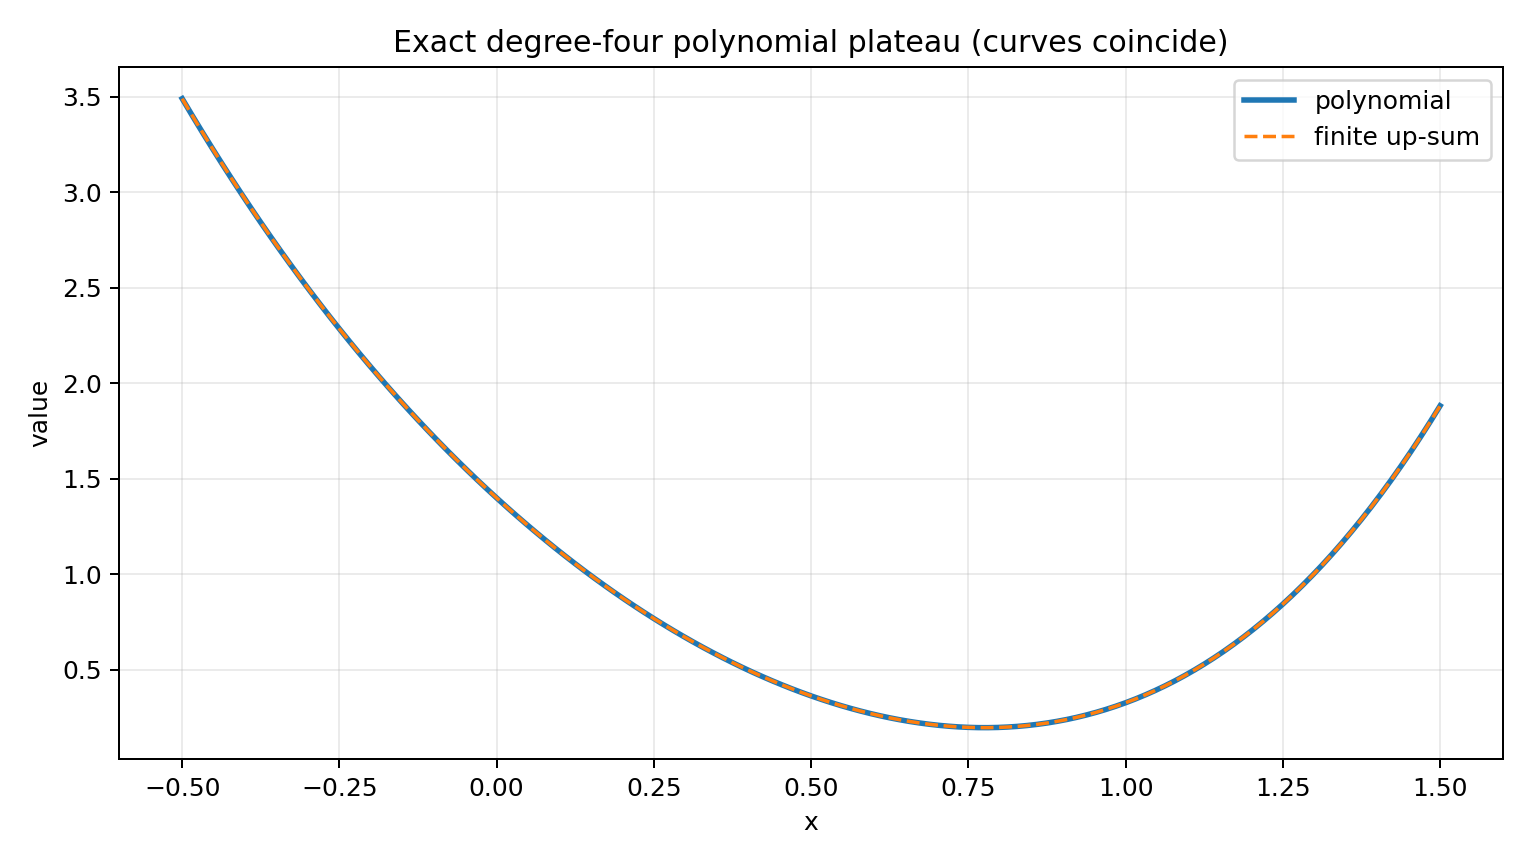
\includegraphics[width=0.92\textwidth]{representation_plot.png}
 \caption{The target polynomial and its finite 49-atom \(\Up\) sum.  The
 displayed numerical curves overlap on \(I\); the identity itself is exact and
 follows from \Cref{thm:finite-plateau}.  Outside \(I\), the compactly supported
 sum is free to leave the polynomial.}
 \label{fig:example}
\end{figure}

The accompanying program evaluates both sides at 129 dyadic points of \(I\)
using exact \texttt{fractions.Fraction} arithmetic for the coefficient
identity.  The maximum residual is the rational number \(0\).  It also
constructs generic examples of degrees \(0,1,\ldots,6\), with canonical
ratios \(1,2,\ldots,64\); every one of the seven exact checks returns zero.
Numerical values of \(\Up\) are used only to draw \Cref{fig:example}, never to
certify the algebra.

\section{Nonuniqueness, canonicality, and null representations}
\label{sec:nonuniqueness}

Finite interval representations are highly nonunique.

\begin{itemize}
  \item Any atom whose support misses \(I\) may be added with arbitrary
        coefficient.
  \item Any finite \(\Up\)-sum vanishing on \(I\) may be added.
  \item The parameters \(m,h,x_0,\rho\) may be changed, subject to
        \(\rho=mh\) and \(\vtwo(m)\ge d\).
  \item The real-space algorithm permits varying scales and different ghost
        placements.
\end{itemize}

The formula of \Cref{alg:main} is nevertheless canonical after fixing
\((m,h,x_0)\): the coefficient polynomial
\(m^{-1}M(\rho\D)^{-1}p\) is uniquely determined.  On the global stationary
space, uniqueness follows from the generating-function calculation: the
coefficient polynomial of degree at most \(d\) is the unique one whose
\(\Up\)-average returns \(p\), by \Cref{prop:prob-characterization}.  The
finite interval truncation then keeps exactly the atoms that can affect \(I\).

This distinction is useful computationally.  One may regard the canonical
formula as a particular solution and the finite sums vanishing on \(I\) as a
nullspace.  Additional objectives---minimum coefficient norm, prescribed
symmetry, sparse scales, endpoint constraints, or integer coefficients after
normalization---can then be posed as optimization in that nullspace without
disturbing exactness.

\section{A generator-independent theorem}
\label{sec:general-generator}

The method is not peculiar to \(\Up\); what is peculiar is the exact dyadic
order law.

\begin{theorem}[Compact-generator Appell reproduction]
\label{thm:general-generator}
Let \(\psi\in C_c^\infty(\R)\) satisfy
\(\int\psi=1\), and put
\[
 M_\psi(z)=\int_\R \e^{zx}\psi(x)\,\dd x.
\]
Fix \(m\in\N_{>0}\).  Suppose that, for every nonzero \(n\in\Z\),
\(\widehat\psi\) has a zero of order at least \(d+1\) at \(mn\).  Define
polynomials \(A_{r,\psi}^{(m)}\) by
\begin{equation}
 \sum_{r\ge0}A_{r,\psi}^{(m)}(u)\frac{z^r}{r!}
 =\frac{\e^{uz}}{mM_\psi(-mz)}.
 \label{eq:general-appell}
\end{equation}
Then, for \(0\le r\le d\),
\begin{equation}
 t^r=\sum_{k\in\Z}A_{r,\psi}^{(m)}(k)
          \psi\!\left(\frac{t-k}{m}\right).
 \label{eq:general-reproduction}
\end{equation}
Consequently every degree-\(d\) polynomial has an exact finite representation
on every compact interval after support truncation.
\end{theorem}

\begin{proof}
Repeat \Cref{lem:twisted-poisson} with \(\psi\).  Dividing by
\(mM_\psi(-mz)\) makes the zero-frequency term \(\e^{tz}\).  The assumed
zero multiplicities kill every nonzero-frequency Taylor coefficient through
degree \(d\).  Coefficient comparison proves
\eqref{eq:general-reproduction}; compact support makes interval restriction
finite.
\end{proof}

For even \(\psi\), \(M_\psi(-z)=M_\psi(z)\), recovering the formulas used
throughout this report.  The theorem also clarifies the exact role of the
infinite sinc product: its nonuniform integer zero multiplicities make the
order depend on the binary valuation of the oversampling ratio.

\section{Tensor-product multivariate extension}
\label{sec:multivariate}

Let
\[
 \Phi(x_1,\ldots,x_s)=\prod_{j=1}^{s}\phi(x_j).
\]
Suppose a polynomial \(p\) has coordinate degree at most \(d_j\) in \(x_j\).
Choose \(m_j\) with \(\vtwo(m_j)\ge d_j\), steps \(h_j>0\), radii
\(\rho_j=m_jh_j\), and origins \(x_{0j}\).  Define
\begin{equation}
 p^\sharp=
 \prod_{j=1}^{s}M(\rho_j\partial_{x_j})^{-1}p.
 \label{eq:multivariate-deconv}
\end{equation}
The commuting differential operators terminate on \(p\).  Tensoring
\Cref{thm:affine-formula} gives
\begin{equation}
 p(\bm x)=
 \frac1{\prod_jm_j}
 \sum_{\bm k\in\Z^s}
 p^\sharp(\bm x_0+\bm k\odot\bm h)
 \prod_{j=1}^{s}
 \phi\!\left(\frac{x_j-x_{0j}-k_jh_j}{\rho_j}\right).
 \label{eq:multivariate-reproduction}
\end{equation}
On a compact box only finitely many multi-indices contribute.  The number of
active atoms at one query point is at most \(\prod_j(2m_j+1)\).  This gives
exact smooth polynomial patches on boxes and, by affine coordinate changes,
on parallelepipeds.

The tensor product is immediate but not necessarily optimal.  A genuinely
multivariate atomic generator with a Fourier zero set adapted to total degree
could avoid the product-of-orders cost.  This is a natural direction for
higher-dimensional Rvachev finite elements.

\section{Further structural consequences}
\label{sec:consequences}

\subsection{Exact smooth localization of polynomial germs}

For every compact interval \(I\), polynomial \(p\), and \(\rho>0\), there is
a compactly supported \(C^\infty\) function in a finite span of equal-scale
\(\Up\)-atoms that equals \(p\) on \(I\) and is supported in
\([A-2\rho,B+2\rho]\).  Unlike multiplication by a generic bump function, the
construction remains inside a prescribed atomic family and gives all
coefficients exactly.

\subsection{Why the mechanism is polynomial-specific}

The nonzero aliases in \eqref{eq:twisted-poisson} have high-order zeros at
\(z=0\), not identically zero germs.  Consequently a finite Taylor jet is
reproduced exactly, while an exponential \(\e^{\lambda t}\) generally retains
nonzero aliases at \(z=\lambda\).  The report therefore does not assert exact
exponential reproduction, nor impossibility for arbitrary varying-scale
finite sums; it isolates the precise stationary obstruction.

\subsection{Piecewise-polynomial targets}

A finite sum of \(\Up\)-atoms is \(C^\infty\).  It cannot equal a target with
a genuine derivative jump at an interior knot.  Separate polynomial pieces
can, however, be represented exactly on closed subintervals separated by
transition gaps, or combined with explicitly chosen smooth transition zones.
If all derivatives match at every knot, a finite piecewise polynomial on a
connected interval is already one polynomial, and the main theorem applies
directly.

\subsection{Moment and derivative duality}

The Appell construction and the Thue--Morse stencil are two sides of one
operator identity.  The Appell coefficients invert the smoothing operator
\(M(\rho\D)\), whose logarithm is an even cumulant series.  The real-space
stencil factors derivatives into dyadic parent--child differences.  In Fourier
space these become, respectively, division by the sinc product near the
origin and multiplication by its zero factors at dyadic frequencies.  Bell
polynomials organize the former; Prouhet--Thue--Morse cancellation organizes
the latter.

\section{Conjectures and frontier questions}
\label{sec:conjectures}

The following statements are plausible consequences or extensions of the
proved theory, but they are not established here.

\begin{conjecturebox}
\textbf{Conjecture 1 (interval-specific dyadic lower bound).}
Fix \(d\ge1\).  There is a length threshold \(L_d\) such that, if a degree-\(d\)
polynomial is represented on an interval of length at least \(L_dh\) by a
finite sum of one-scale atoms
\(\phi((x-kh-x_0)/(mh))\) with arbitrary coefficients and with no atoms
identically zero on the interval, then \(\vtwo(m)\ge d\).  Thus sufficiently
long exact plateaux cannot beat the stationary binary order by boundary
engineering.
\end{conjecturebox}

\begin{conjecturebox}
\textbf{Conjecture 2 (exponential atom complexity).}
For intervals whose length is comparable to the atom radius and under a
uniform bound on support enlargement, every one-scale exact representation of
all degree-\(d\) polynomials requires \(\Omega(2^d)\) atoms in the worst case.
The canonical construction, with \(2^{d+1}+\bigO(1)\) boundary atoms, would
then be order-optimal.
\end{conjecturebox}

\begin{conjecturebox}
\textbf{Conjecture 3 (stable-radius principle).}
For each fixed polynomial and interval, the coefficient norm of the canonical
representation has a finite minimizing radius \(\rho_*>0\).  After affine
normalization of the interval, \(\rho_*\) is controlled by the nearest complex
critical scale of the inverse symbol \(1/M(\rho z)\), and varies continuously
with the polynomial away from degree drops.
\end{conjecturebox}

\begin{conjecturebox}
\textbf{Conjecture 4 (ghost/Appell variational limit).}
Apply the real-space antiderivative algorithm on successively larger symmetric
working intervals and choose the \(\ell^2\)-optimal ghost split
\eqref{eq:l2-ghost} at every level.  After matching the final scale and lattice,
the interior coefficient sequences converge to the canonical Appell samples
of \Cref{alg:main}.
\end{conjecturebox}

\begin{conjecturebox}
\textbf{Conjecture 5 (local extended-Chebyshev behavior).}
For generic ordered centers and a sufficiently short interval avoiding all
support endpoints, a finite family of equal-scale \(\Up\)-translates forms an
extended Chebyshev system.  If true, local interpolation matrices would be
strictly sign-regular and the null representations discussed in
\Cref{sec:nonuniqueness} would arise only after the interval crosses a
generator-dependent length threshold.
\end{conjecturebox}

\begin{conjecturebox}
\textbf{Conjecture 6 (sharp odd-denominator law).}
After removing the evident factor \(m^{r-1}\), the reduced denominator of
\(A_r^{(m)}(u)\) at dyadic \(u\) has a \(2\)-adic valuation determined solely
by the dyadic denominator of \(u\) and the binary digit sums of the Bell
partitions of \(r\).  All irregular prime growth is confined to odd primes
dividing numbers \(2^{2j}-1\) and Bernoulli numerators.
\end{conjecturebox}

\begin{conjecturebox}
\textbf{Conjecture 7 (endpoint-scale lower-Lambert asymptotics).}
Let \(P_d(u)=A_d^{(1)}(u)\).  In the boundary scaling
\(u=1+\delta_d\), with \(\delta_d2^d/d\) bounded away from both zero and
infinity, the dominant positive-real saddle \(z_d\) obeys
\[
 d=\delta_d z_d+\log_2 z_d+\Theta(1).
\]
The full asymptotic expansion of \(P_d(1+\delta_d)\) contains a nonconstant
one-periodic function of the corresponding lower-Lambert phase, analogous to
the periodic correction in the Fabius endpoint asymptotic.  Fixed-\(u\)
coefficients, by contrast, are governed by the nearest imaginary poles of
\(1/M\).
\end{conjecturebox}

\begin{conjecturebox}
\textbf{Conjecture 8 (\(q\)-geometric atomic reproduction).}
There is a nonstationary atomic family with geometrically varying scales whose
exact derivative and reproduction stencils have coefficients
\((-1)^rq^{\binom r2}\qbinom{d}{r}{q}\).  At \(q=2\) it should interact with
the Rvachev refinement equation, while the limit \(q\to1\) recovers ordinary
finite differences and classical Appell reproduction.
\end{conjecturebox}

\section{Promising research directions}
\label{sec:future}

\subsection{Lean formalization}

A compact formalization path is:
\begin{enumerate}
  \item prove the exact integer zero multiplicity of the sinc product;
  \item formalize twisted Poisson summation for a smooth compactly supported
        function with an exponential twist;
  \item define the finite-degree inverse \(M(m\D)^{-1}\) in
        \(\Q[\D]/(\D^{d+1})\);
  \item prove the Appell generating identity and coefficient comparison;
  \item derive the affine finite-interval truncation and support bounds;
  \item formalize the parent--child derivative identity, finite prefix-sum
        primitive, and Thue--Morse stencil.
\end{enumerate}
Most analytic difficulty is concentrated in Poisson summation; the remaining
steps are finite polynomial algebra and exact support reasoning.

\subsection{Certified symbolic software}

The Python prototype should be developed into a small exact library that:
accepts rational or algebraic input; emits a compressed coefficient polynomial
or an expanded atom table; optimizes \(\rho\) under support and norm
constraints; evaluates \(\Up\) at dyadic points with the repository's exact
algorithm; and exports Lean-checkable certificates consisting of moment
recurrences, polynomial identities, and support inequalities.

\subsection{Minimal varying-scale representations}

The common-scale theorem is explicit but probably not atom-minimal.  The
real-space construction suggests a mixed-integer problem over a dyadic tree:
select parent atoms, ghost leaves, and scale transitions so that derivative
constraints telescope while minimizing atom count or coefficient norm.
Lower bounds could combine local linear independence, support geometry, and
Fourier zero multiplicities.

\subsection{Atomic finite elements and exact patch tests}

Polynomial reproduction is the mathematical core of a finite-element patch
test.  Tensor products of the present plateaux give compactly supported
\(C^\infty\) shape-function combinations that pass every prescribed
polynomial patch test exactly.  Useful next questions include sparse
multivariate generators, boundary-adapted bases, exact quadrature, stiffness
matrix arithmetic, and condition numbers relative to conventional
high-order splines.

\subsection{Asymptotics of the Appell table}

The generating function \(\e^{uz}/M(z)\) offers several asymptotic regimes:
nearest-pole expansions for fixed \(u\), saddle-point behavior when \(u\)
grows with degree, and the delicate endpoint scale
\(u=\pm1+\bigO(d2^{-d})\), where the exponential type of \(M\) nearly
cancels the numerator.  Mellin analysis of \(\log M\), inverse lower-Lambert
coordinates, and periodic fluctuations from the dyadic product should connect
this coefficient problem directly to the repository's endpoint machinery.

\section{Summary of proved results}
\label{sec:summary}

\begin{resultbox}
For every polynomial \(p\) of degree \(d\), every compact interval
\(I=[A,B]\), every \(x_0\in\R\), and every \(\rho>0\), choose
\(m=2^d\) and \(h=\rho/m\).  Then
\[
 p(x)=\frac1m
 \sum_{k=\ceil{(A-x_0)/h-m}}^{\floor{(B-x_0)/h+m}}
 \bigl[M(\rho\D)^{-1}p\bigr](x_0+kh)
 \Up\!\left(\frac{x-x_0-kh}{\rho}\right)
 \qquad(x\in[A,B]).
\]
The sum is finite, uses one common scale, has rational coefficients for
rational data, matches every endpoint jet, and is supported in
\([A-2\rho,B+2\rho]\).  Its atom count is at most
\[
 \floor{m\left(\frac{B-A}{\rho}+2\right)}+1.
\]
For an arbitrary positive integer \(m\), the exact stationary reproduction
degree is precisely \(\vtwo(m)\); the next degree has the explicit nonzero
alias defect \eqref{eq:first-defect}.  The inverse symbol is governed by the
Bernoulli cumulants \eqref{eq:kappa}, while repeated real-space
differentiation produces the Thue--Morse stencil
\eqref{eq:thue-morse-stencil}.
\end{resultbox}

\appendix

\section{Exact dyadic values used for independent checks}
\label{app:dyadic}

The numerical plot evaluates \(\Up\) through the bounded Fabius function
\(F\), using \(\Up(x)=F(1-\abs{x})\) for \(\abs{x}\le1\).  One exact dyadic
formula compatible with the repository normalization is
\begin{equation}
 F\!\left(\frac{a}{2^n}\right)
 =
 \frac{2^{-\binom{n+1}{2}}}{n!}
 \sum_{j=0}^{a-1}(-1)^{\wt(j)}
 \sum_{r=0}^{\floor{n/2}}
 \binom n{2r}\mu_{2r}(2a-2j-1)^{n-2r},
 \label{eq:dyadic-fabius}
\end{equation}
for \(0\le a\le2^n\), with the endpoint conventions \(F(0)=0\),
\(F(1)=1\).  Reduction to lowest terms is performed after the integer and
moment sums are complete.  This formula supplies exact reference values; the
proof of polynomial reproduction itself does not depend on pointwise
evaluation of \(F\) or \(\Up\).

\section{Archive manifest and reproducibility}
\label{app:manifest}

The ZIP archive contains:
\begin{longtable}{>{\raggedright\arraybackslash}p{0.42\textwidth}p{0.52\textwidth}}
\toprule
File & Purpose\\
\midrule
\endhead
\path{Exact_Polynomial_Plateaux_from_Rvachev_Up.tex}
& Complete LaTeX source of this report.\\
\path{Exact_Polynomial_Plateaux_from_Rvachev_Up.pdf}
& Rendered report.\\
\path{rvachev_polynomial_reproduction.py}
& Commented exact-arithmetic construction, verification, CSV generation, and
  plotting code.\\
\path{example_coefficients.csv}
& All 49 rational coefficients of \eqref{eq:example-representation}.\\
\path{exact_grid_check.csv}
& Exact values and residuals at 129 dyadic test points.\\
\path{appell_coefficients_m16.csv}
& Coefficient table for \(A_r^{(16)}\), \(0\le r\le8\).\\
\path{generic_degree_checks.csv}
& Independent exact checks for degrees \(0\) through \(6\).\\
\path{verification_summary.txt}
& Human-readable zero-residual summary.\\
\path{representation_plot.png}
& Figure used in \Cref{fig:example}.\\
\path{README.md}
& Reproduction instructions and normalization notes.\\
\path{SHA256SUMS}
& Integrity hashes for the packaged files.\\
\bottomrule
\end{longtable}

Run
\begin{lstlisting}[style=pseudo]
python rvachev_polynomial_reproduction.py
latexmk -pdf -interaction=nonstopmode \
  -halt-on-error Exact_Polynomial_Plateaux_from_Rvachev_Up.tex
\end{lstlisting}
from the unpacked directory.  The script uses only the Python standard library
for exact algebra; Matplotlib is used for the optional figure.

\section{Notation crosswalk}
\label{app:notation}

\begin{center}
\begin{tabularx}{\textwidth}{@{}lX@{}}
\toprule
Symbol & Meaning\\
\midrule
\(\phi=\Up\) & Even Rvachev up-function supported on \([-1,1]\).\\
\(F\) & Bounded Fabius distribution function on \([0,1]\), extended by
constants outside.\\
\(M(z)\) & Moment-generating function \(\int\e^{zx}\phi(x)\,\dd x\).\\
\(\kappa_{2r}\) & Even cumulants of the probability density \(\phi\).\\
\(A_r^{(m)}\) & Up-Appell polynomial defined by \eqref{eq:appell-egf}.\\
\(h\) & Lattice spacing between atom centers.\\
\(m\) & Integer radius-to-spacing ratio.\\
\(\rho=mh\) & Physical radius/scale of each atom.\\
\(p_\rho^\sharp\) & Exact deconvolution \(M(\rho\D)^{-1}p\).\\
\(\wt(k)\) & Number of one-bits in the binary expansion of \(k\).\\
\(\vtwo(k)\) & Exponent of two dividing a nonzero integer \(k\).\\
\bottomrule
\end{tabularx}
\end{center}

\begin{thebibliography}{99}

\bibitem{repo-primary}
V.~Reshetnikov,
\emph{Fabius Function and Rvachev Up},
in the ProveIt repository, directory
\texttt{Analysis/FabiusFunction/docs/Fabius\_Function\_and\_Rvachev\_Up},
snapshot of 28 August 2026.

\bibitem{repo-frontier}
V.~Reshetnikov,
\emph{Non-formalized Research Frontiers for the Fabius/Rvachev Development},
in the ProveIt repository, directory
\texttt{Analysis/FabiusFunction/docs/non-formalized-research-frontiers},
snapshot of 28 August 2026.

\bibitem{repo-sampling}
V.~Reshetnikov,
\emph{Inverse and Sampling Frontiers for the Fabius--Rvachev System},
in the ProveIt repository, directory
\texttt{Analysis/FabiusFunction/docs/non-formalized-research-frontiers/
 drafts/inverse-and-sampling/Inverse\_and\_Sampling\_Frontiers},
commit \texttt{5915d9a723c9ae01a2cc4be8a251bdcb11d9e406}, 28 August 2026.

\bibitem{repo-glossary}
V.~Reshetnikov,
\emph{Mathematical Glossary for Analysis/FabiusFunction},
in the ProveIt repository, directory
\texttt{Analysis/FabiusFunction/docs/FabiusFunction\_Mathematical\_Glossary},
snapshot of 28 August 2026.

\bibitem{arias}
J.~Arias de Reyna,
\emph{An infinitely differentiable function with compact support: Definition
and properties},
arXiv:1702.05442, 2017; English translation of the 1982 paper.

\bibitem{rvachev}
V.~L.~Rvachev,
\emph{Theory of \(R\)-Functions and Some Applications},
Naukova Dumka, Kyiv, 1982 (in Russian).

\bibitem{strangfix}
G.~Strang and G.~Fix,
A Fourier analysis of the finite element variational method,
in \emph{Constructive Aspects of Functional Analysis},
Cremonese, Rome, 1973, pp.~793--840.

\bibitem{dahmenmicchelli}
W.~Dahmen and C.~A.~Micchelli,
Translates of multivariate splines,
\emph{Linear Algebra and its Applications} \textbf{52/53} (1983),
217--234.

\bibitem{zakharov}
V.~Zakharov,
Polynomial spaces reproduced by elliptic scaling functions,
arXiv:1310.8425, 2013.

\bibitem{deboorron}
C.~de Boor, R.~A.~DeVore, and A.~Ron,
The structure of finitely generated shift-invariant spaces in
\(L_2(\R^d)\),
\emph{Journal of Functional Analysis} \textbf{119} (1994), 37--78.

\bibitem{comtet}
L.~Comtet,
\emph{Advanced Combinatorics},
D. Reidel, Dordrecht, 1974.

\bibitem{jessenwintner}
B.~Jessen and A.~Wintner,
Distribution functions and the Riemann zeta function,
\emph{Transactions of the American Mathematical Society}
\textbf{38} (1935), 48--88.

\bibitem{haugland}
J.~K.~Haugland,
Evaluating the Fabius function,
arXiv:1609.07999, 2016.

\end{thebibliography}

\end{document}
